\documentclass[aspectratio=169, table]{beamer}
\usepackage[utf8]{inputenc}
\usepackage[T1]{fontenc}
\usepackage{graphicx}
\usepackage{fontspec}
\usepackage{xcolor}
\usepackage{tcolorbox}
\usepackage{listings} % Add the listings package
\usepackage{hyperref} % Add the hyperref package
\usepackage{booktabs}

\lstdefinelanguage{JavaScript}{
    keywords={function, var, let, const, if, else, for, while, return, true, false},
    keywordstyle=\color{blue}\bfseries,
    ndkeywords={class, export, boolean, throw, implements, import, this},
    ndkeywordstyle=\color{orange}\bfseries,
    identifierstyle=\color{black},
    sensitive=false,
    comment=[l]{//},
    morecomment=[s]{/*}{*/},
    commentstyle=\color{gray}\ttfamily,
    stringstyle=\color{green}\ttfamily,
}

\lstdefinelanguage{CSS}{
    keywords={color, background, margin, padding, font-size, text-align, border},
    keywordstyle=\color{blue}\bfseries,
    ndkeywords={url},
    ndkeywordstyle=\color{orange}\bfseries,
    identifierstyle=\color{black},
    sensitive=false,
    comment=[l]{//},
    morecomment=[s]{/*}{*/},
    commentstyle=\color{gray}\ttfamily,
    stringstyle=\color{green}\ttfamily,
}

\lstset{
    breaklines=true,
    language=JavaScript,
    % ... (other style settings)
}

\setsansfont[
  ItalicFont=fonts/TitilliumWeb-Italic.ttf,
  BoldFont=fonts/TitilliumWeb-Bold.ttf,
  BoldItalicFont=fonts/TitilliumWeb-BoldItalic.ttf,
]{TitilliumWeb-Regular.ttf}

\subtitle{IF120203-Web Programming}
\title{\huge {\textbf{06: Responsive\\Website}}}
\date[Serial]{\scriptsize {PRU/SPMI/FR-BM-18/0222}}
\author[Pradita]{\small {\textbf{PRADITA UNIVERSITY}}}

\usetheme{Pradita}

\begin{document}
\begin{frame}
    \titlepage
\end{frame}

\begin{frame}{Goals for Today}
    \vskip-1cm
    \begin{itemize}
        \item To grasp the core concepts of responsive design
        \item To understand the concept of using media queries and breakpoints
        \item To understand how to make responsive design by using Bootstrap 
        \item To develop a website with cross-browser and cross-device compatibility
    \end{itemize}
\end{frame}

\begin{frame}{Introduction to Responsive Web}
    \vskip1cm
    \begin{itemize}
        \item Responsive web design is the approach of creating websites that automatically adapt and adjust their layout and content to different screen sizes, such as those of smartphones, tablets, laptops, and desktops. This ensures that users can easily access and navigate the website, regardless of the device they are using.
    \end{itemize}
    \begin{center}
	
\includegraphics[width=0.5\textwidth]{classFiles/responsive-web.png}
    \end{center}
\end{frame}

\begin{frame}[fragile]
	\frametitle{Introduction to Breakpoints}
	\vskip0cm
	 \begin{itemize}
        \item Think of breakpoints as points where your website's layout changes to fit different screen sizes. It's like having a special plan for how your website looks on phones, tablets, and computers.
	\item Imagine you're drawing a picture on a piece of paper. When the paper gets too small, you might need to start drawing smaller pictures. Breakpoints are like those moments when you decide to draw a new picture because the space you have is different.
   	 \end{itemize}
\end{frame}

\begin{frame}[fragile]
	\frametitle{Introduction to Breakpoints}
	\vskip1cm
	\begin{center}
		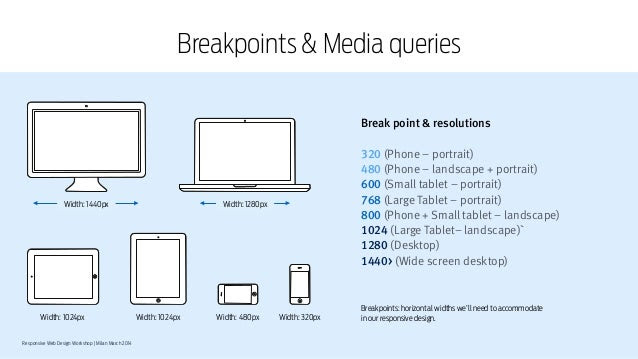
\includegraphics[width=0.8\textwidth]{classFiles/breakpoints.jpg}
	\end{center}
\end{frame}

\begin{frame}[fragile]
	\frametitle{Introduction to Media Queries}
	\vskip1cm
	 \begin{itemize}
        \item Media queries are like instructions you give to your website to do something different at certain points. It's like saying, "Hey website, when the screen is this size, do this thing!"
	\item Imagine you have a robot friend. You tell the robot, "When it's sunny outside, bring me an umbrella." Media queries are like those instructions you give to your website, telling it how to change things based on the screen size.
   	 \end{itemize}
\end{frame}

\begin{frame}[fragile]
	\frametitle{Introduction to Media Queries}
	\vskip0cm
	\begin{center}
		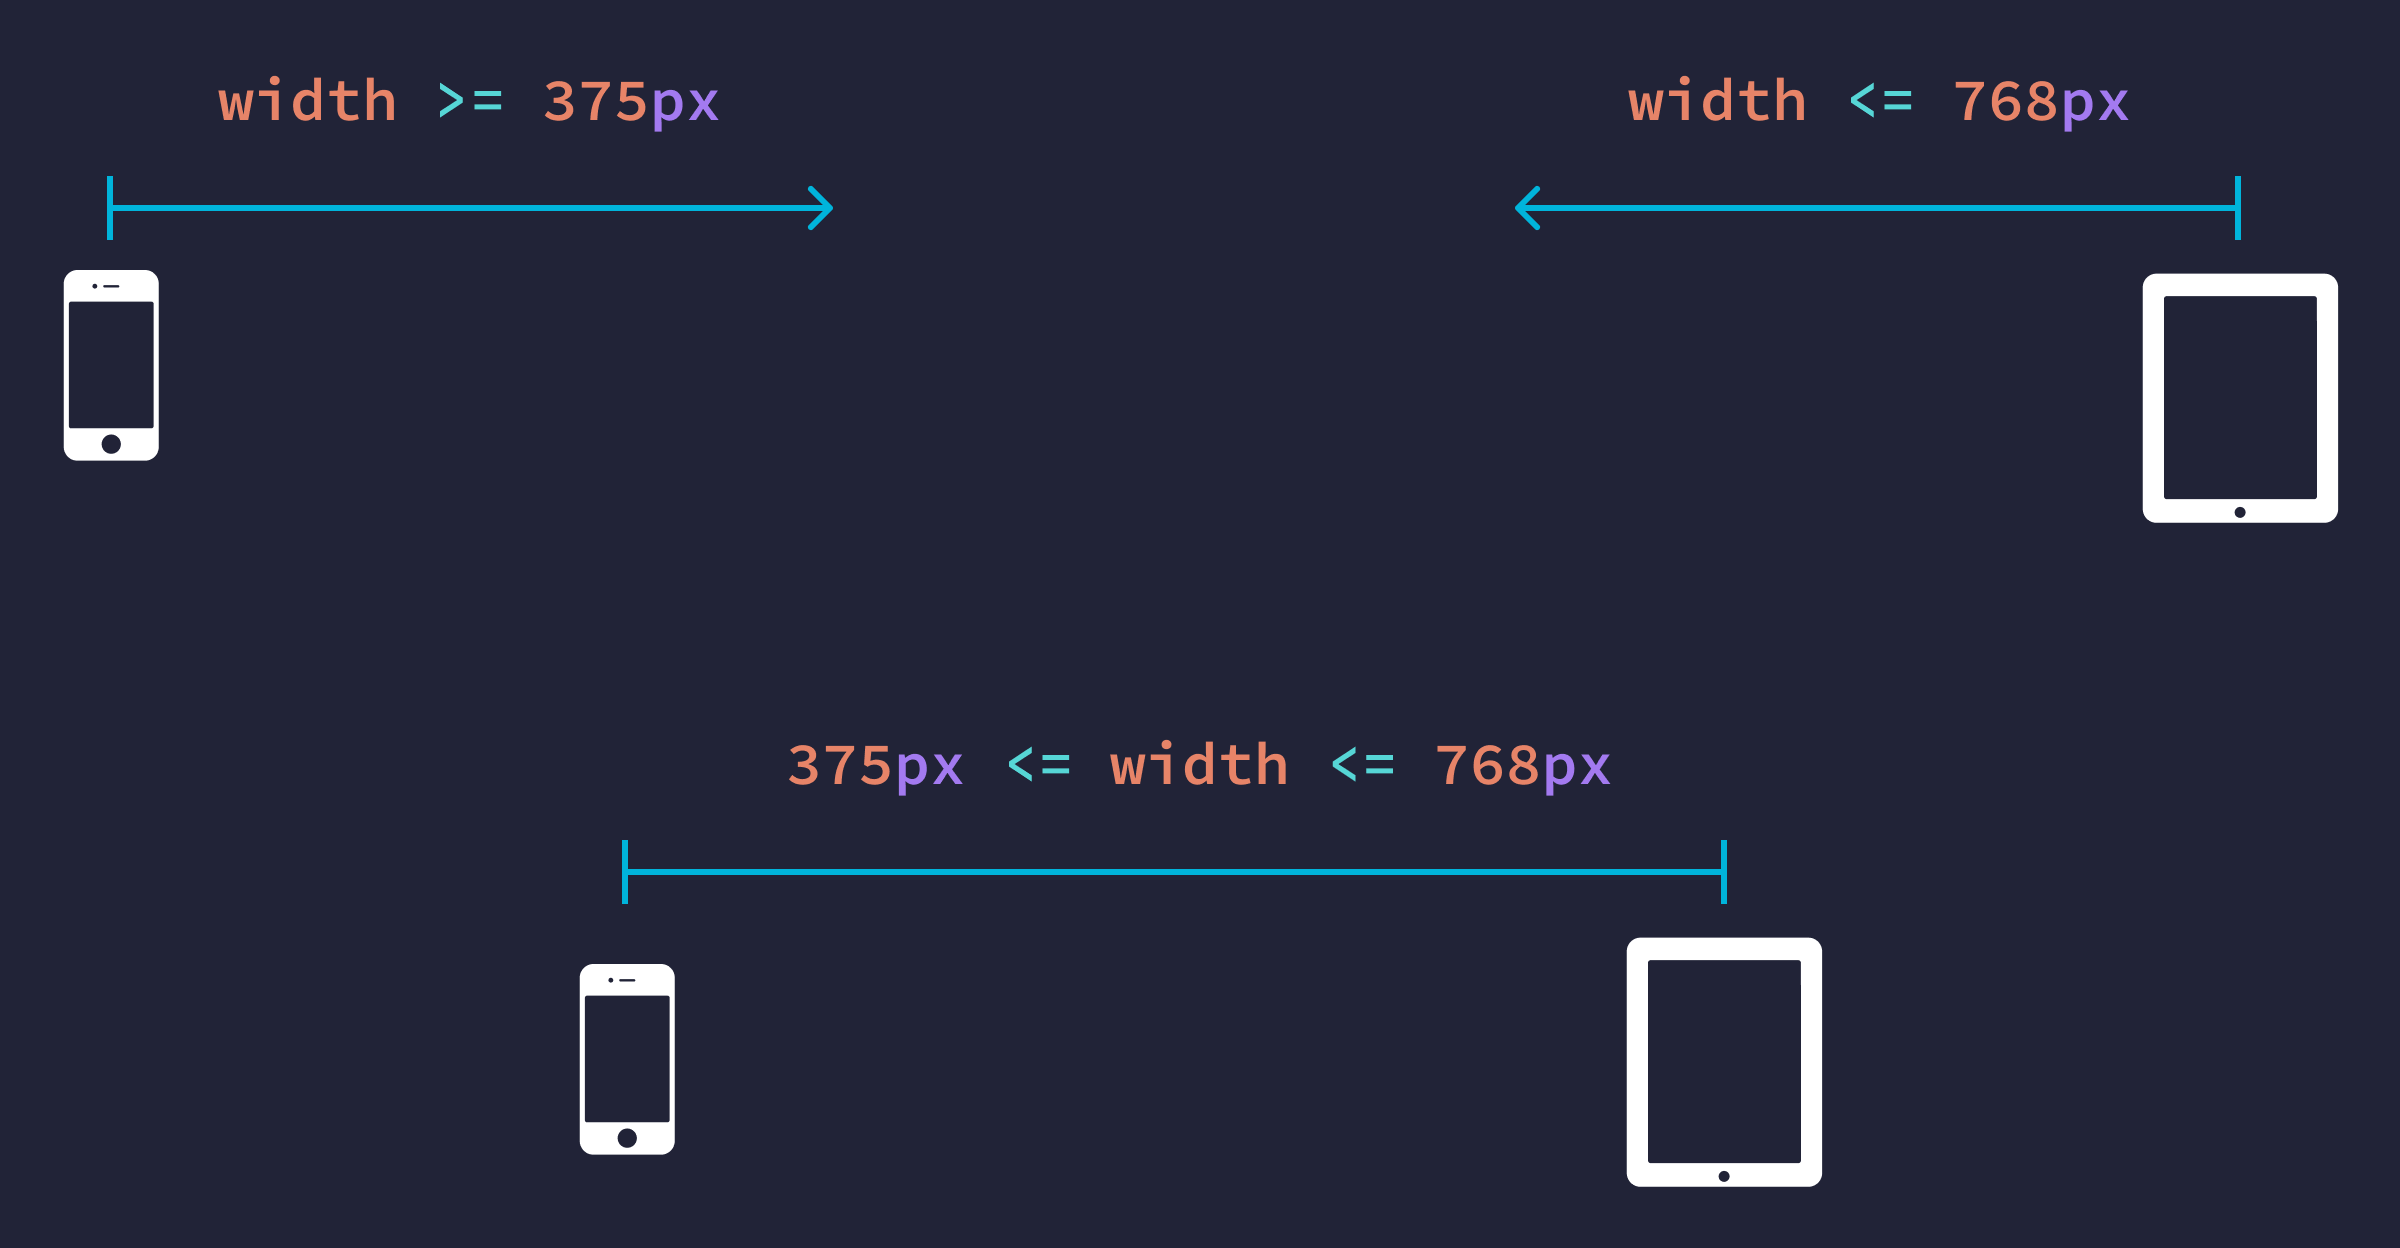
\includegraphics[width=0.8\textwidth]{classFiles/media-queries.png}
	\end{center}
\end{frame}

\begin{frame}[fragile]
	\frametitle{Bootstrap and Breakpoints}
	\vskip0cm
	 \begin{itemize}
        \item Bootstrap is like a helper for building websites. It comes with its own breakpoints that you can use. It's like having a coloring book with lines already drawn for you to color within.
	\item Bootstrap knows when to switch things around for different screen sizes. For example, it might make buttons bigger on phones so you can tap them easily, and smaller on computers where you have a mouse.
	\item Source: https://getbootstrap.com/docs/5.3/layout/grid/
   	 \end{itemize}
\end{frame}

\begin{frame}[fragile]
	\frametitle{Bootstrap Grid Classes}
	\vskip1cm
	 \begin{itemize}
        \item xs (for phones - screens less than 575px wide)
	\item .col- (extra small devices - screen width less than 576px)
	\item .col-sm- (small devices - tablets - screen width equal to or greater than 576px)
	\item .col-md- (medium devices - small laptops - screen width equal to or greater than 768px)
	\item .col-lg- (large devices - laptop and desktops - screen width equal to or greater than 992px)
	\item .col-xl- (xlarge devices - laptops and desktops - screen width equal to or greater than 1200px)
   	 \end{itemize}
\end{frame}

\begin{frame}[fragile]
	\frametitle{Bootstrap Grid Classes}
	\vskip1.5cm
	 \begin{itemize}
        \item To create the layout you want, create a container (<div class="container">). Next, create a row (<div class="row">). Then, add the desired number of columns (tags with appropriate .col-*-* classes). Note that numbers in .col-*-* should always add up to 12 for each row.
   	 \end{itemize}
	\begin{center}
		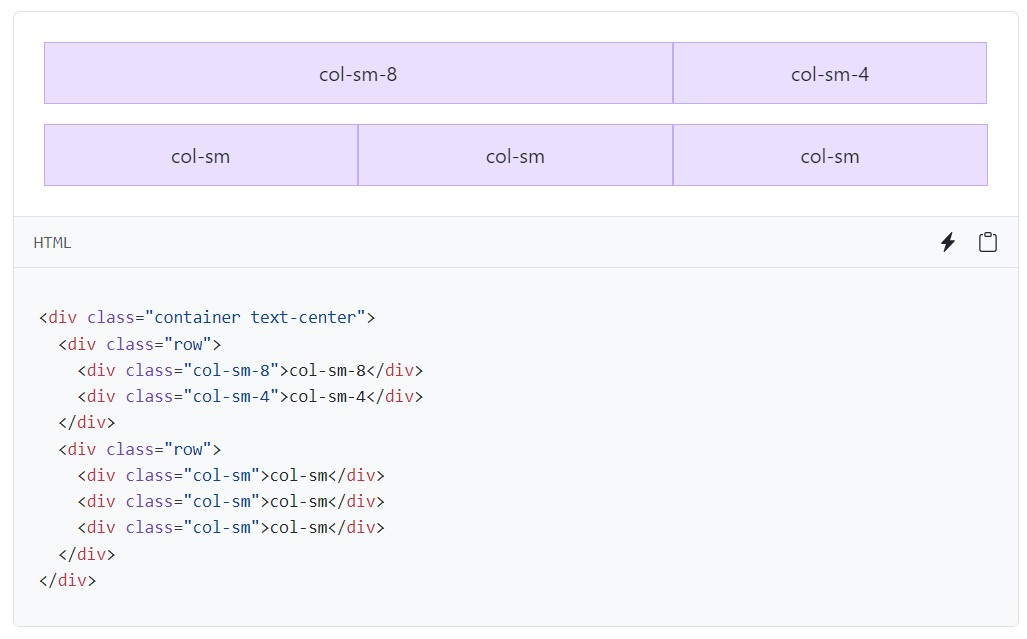
\includegraphics[width=0.5\textwidth]{classFiles/bootstrap-grid.jpg}
	\end{center}
\end{frame}


% ... (previous frames)

\begin{frame3}
    \vskip1cm
    \begin{tcolorbox}[standard jigsaw, opacityback=0, opacityframe=0, sharp corners, boxrule=0pt]
        \begin{columns}[T] %T for Top, C for Center, B for Bottom
            \begin{column}{0.5\textwidth}	
                \begin{center}
                	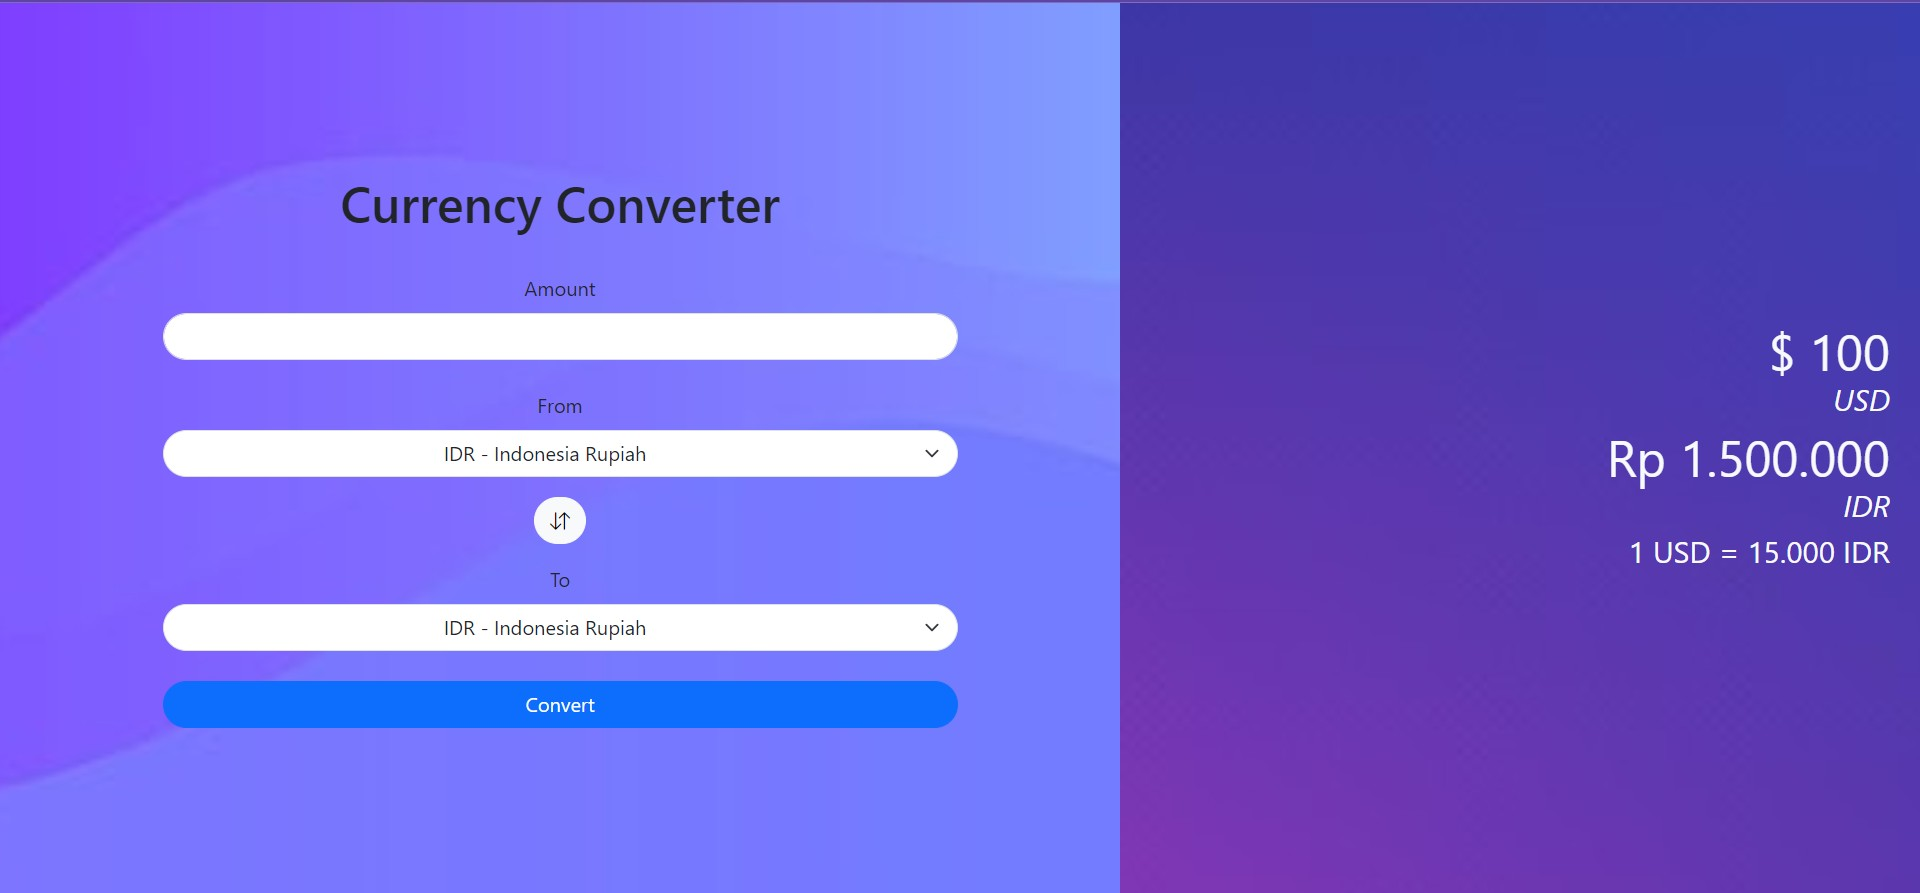
\includegraphics[width=1\textwidth]{classFiles/responsive-currency-converter.jpg}
		\end{center}
            \end{column}
            \begin{column}{0.5\textwidth}
		\begin{center}
                	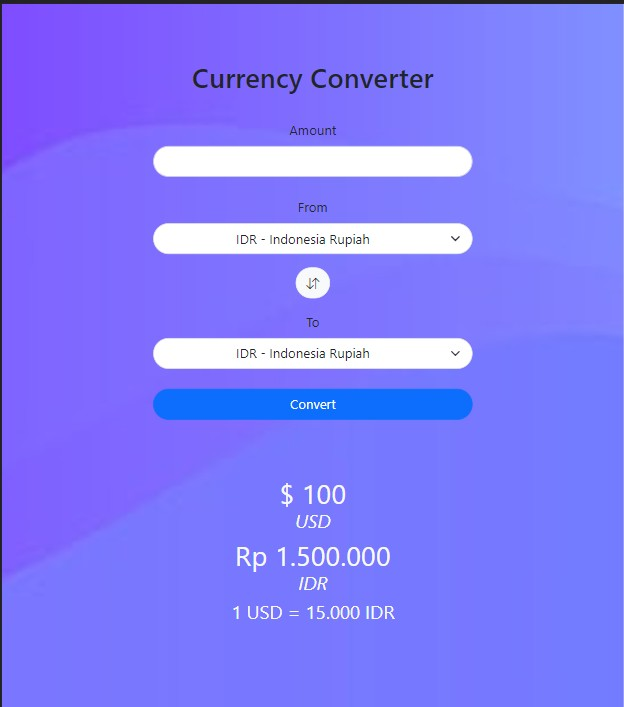
\includegraphics[width=0.7\textwidth]{classFiles/responsive-currency-converter-mobile.jpg}
		\end{center}
            \end{column}
        \end{columns}
    \end{tcolorbox}
\end{frame3}


\begin{frame}[fragile]
    \frametitle{Update Code - HTML - 1}
    \vskip1cm
    \begin{lstlisting}[language=HTML]
<div class="row">
    <div class="col-7 left-section d-flex flex-column align-items-center justify-content-center">
      <div class="container-fluid d-flex flex-column align-items-center justify-content-center gap-4">
    \end{lstlisting}
 	
	\begin{itemize}
        \item Change it to code below
   	 \end{itemize}

\begin{lstlisting}[language=HTML]
  <div class="row min-vh-100">
    <div class="col-md-7 col-12 left-section d-flex flex-column align-items-center justify-content-center">
      <div class="container d-flex flex-column align-items-center justify-content-center gap-4">
    \end{lstlisting}
\end{frame}


\begin{frame}[fragile]
    \frametitle{Update Code - HTML - 2}
    \vskip1cm
    \begin{lstlisting}[language=HTML]
<div class="col-5 right-section d-flex flex-column justify-content-center text-light">
  <div class="container-fluid d-flex flex-column justify-content-center text-light">
    <div class="result-wrapper d-flex flex-column align-items-end">
    \end{lstlisting}
 	
	\begin{itemize}
        \item Change it to code below
   	 \end{itemize}

\begin{lstlisting}[language=HTML]
<div class="col-md-5 col-12 right-section d-flex flex-column justify-content-md-center justify-content-start text-light">
  <div class="container d-flex flex-column justify-content-center text-light">
    <div class="result-wrapper d-flex flex-column align-items-md-end align-items-center">
    \end{lstlisting}
\end{frame}


\begin{frame}[fragile]
    \frametitle{Update Code - HTML - 3}
    \vskip1cm
    \begin{lstlisting}[language=HTML]
<div class="result-wrapper d-flex flex-column align-items-end">
    \end{lstlisting}
 	
	\begin{itemize}
        \item Change it to code below
   	 \end{itemize}

\begin{lstlisting}[language=HTML]
<div class="result-wrapper d-flex flex-column align-items-md-end align-items-center">
    \end{lstlisting}
\end{frame}

\begin{frame}[fragile]
    \frametitle{Update Code - HTML - 4}
    \vskip1cm
    \begin{lstlisting}[language=HTML]
<label class="exchange-rate d-flex flex-column align-items-end h4 fw-normal" id="exchange-rate">1 USD = 15.000 IDR</label>
    \end{lstlisting}
 	
	\begin{itemize}
        \item Change it to code below
   	 \end{itemize}

\begin{lstlisting}[language=HTML]
<label class="exchange-rate d-flex flex-column align-items-md-end align-items-center h4 fw-normal" id="exchange-rate">1 USD = 15.000 IDR</label>
    \end{lstlisting}
\end{frame}

\begin{frame}[fragile]
    \frametitle{Update Code - CSS - 1}
    \vskip1cm
	\begin{itemize}
        \item Add this
   	 \end{itemize}

\begin{lstlisting}[language=CSS]
@media (max-width: 767px) {
  body {
    background-image: url("../img/left-background.png");
    background-size: cover;
    background-position: center;
    background-repeat: no-repeat;
    min-height: 100vh;
  }

/* To be continued */

}

    \end{lstlisting}
\end{frame}

\begin{frame}[fragile]
    \frametitle{Update Code - CSS - 2}
    \vskip1cm
	\begin{itemize}
        \item Add this
   	 \end{itemize}

\begin{lstlisting}[language=CSS]
@media (max-width: 767px) {
/* Continuing... */
.left-section {
    min-height: 0vh;
    background-image: none;
    width: 100%;
    padding: 20px;
  }

  .right-section {
    margin-top: 0;
    background-image: none;
    min-height: 0vh;
  }
}

    \end{lstlisting}
\end{frame}



\begin{frame4}
    \frametitle{Thank You}
\end{frame4}

\end{document}
